\chapter{Familiarisation with Capacitor}

\section{Aim}
	The main objectives are as per following:
	\begin{itemize}
		\tightlist
		\item Provide a definition of capacitor and name its units
		\item Explain how a capacitor can be constructed to give a particular value of capacitance
		\item Determine experimentally the energy stored in a capacitor
		\item Identify the value and type of capacitor
		\item Identify the polarity of terminals
	\end{itemize}

\section{Apparatus}
	\begin{itemize}
		\tightlist
		\item Ceramic Capacitor ($1000\mu F$)
		\item Electrolytic Capacitor ($1000 \mu F$)
		\item Ammeter
		\item Bulb
		\item Switch
		\item 12V Battery
	\end{itemize}

\section{Theory}
	\subsection{What is a Capacitor}		
		\begin{figure}[h!]
			\centering
			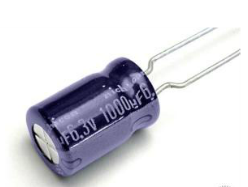
\includegraphics[width=0.7\linewidth]{img/exp2/1}
			\caption[]{A simple ceramic capacitor}
			\label{fig:cap1}
		\end{figure}
		It is one of the passive components like resistor. Capacitor is also known as condenser. Capacitor is generally used to store the charge. The charge is stored in the form of “electrical field”. Capacitors play a major role in many electrical and electronic circuits.
	
	\subsection{Construction of a Capacitor}
		The basic construction of all capacitors is of two parallel metal plates separated by an insulating material (Figure \ref{fig:capcons:1}). An insulator is a material which is non-conducting i.e. it shows a high resistance to letting to electric used is air, other types are oil or paper. Real capacitors are made by taking thin strips of metal foil and the appropriate dielectric material and sandwiching them together.
		
		\begin{figure}[ht]
			\centering 
			\subfloat[Metallic plates of a capacitor]{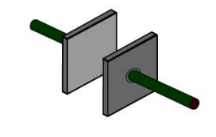
\includegraphics[width=0.45\textwidth,valign=c]{img/exp2/2}
				\label{fig:capcons:1}}	
			\hfill
			\subfloat[Increasing the area of capacitor by wounding]{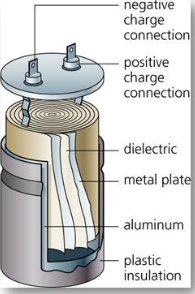
\includegraphics[width=0.45\textwidth,valign=c]{img/exp2/3}
				\label{fig:capcons:2}}			
			\caption{\textit{Internal view of a simple capacitor}}
		\end{figure}
	
		Capacitor achieve large area (thus large capacitance) by doing something tricky, such as putting a dielectric between 2 layers of metal foil and rolling it up like in Figure \ref{fig:capcons:2}.

	\subsection{Capacitance}
		A capacitor is so called because it has the capacity to store charge- just like a beaker storing a liquid. Capacitors are marked with a value which indicates their capacitance – their ability to store charge . Capacitance can be thought of as the “electrical capacity” of that body. It is measured in Farads.
		\begin{figure}[h!]
			\centering
			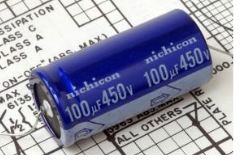
\includegraphics[width=0.5\linewidth]{img/exp2/4}
			\caption[]{A capacitor with $100\mu F$ capacitance}
			\label{fig:cap2}
		\end{figure}
	
	\subsection{Maximum Working Voltage}
		If the voltage across a capacitor is too high, the insulator between the plates fails to insulate and charge passes from one plate to the other . Capacitor are usually marked with the maximum working voltage to help the user avoid situation.\\
		A good rule of thumb is to never place a voltage across the capacitor which exceeds about two thirds of this value, especially for alternating current circuits.
		
	\subsection{Mathematical Notation}
		A static description of the way a capacitor behaves would be to say $Q=C \times V$, where $Q$ is the total charge, $C$ is a measure of how big the capacitor is and $V$ is the voltage across it.\\
		\\
		A dynamic description ,ie one that changes with time would be to say $I = C \times\frac{dV}{dt}$ . This is just the time derivative of the static description.$C$ is constant wrt time, $I$ is the rate at which charge flows . This essentially says – the bigger the current , the faster the capacitor’s voltage changes.
		
				
	\subsection{Classification of Capacitor}
		\textbf{Polarized}: They have positive and negative electrode.\\
		\textbf{Un-Polarized}: They don't have positive and negative electrode
		\begin{table}[h]
			\centering
			\begin{tabular}{|l|l|}
				\hline
				\textbf{UN-POLARIZED} & \textbf{POLARIZED} \\
				\hline
				Ceramic & Electrolytic \\
				\hline
				Multilayer & Tantalum \\
				\hline
				Polystyrene Film & Super \\
				\hline
				Polyster Film &  \\
				\hline
				Polypropylene &  \\
				\hline
				Mica &  \\
				\hline
			\end{tabular}
		\caption{Examples of Polarized and Un-Polarized Capacitors}
		\end{table}
		
		\subsubsection{Ceramic Capacitors}
			\begin{figure}[h]
				\centering
				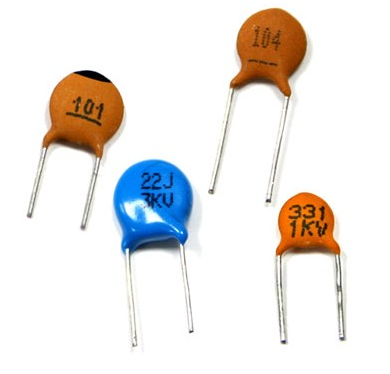
\includegraphics[width=0.5\linewidth]{img/exp2/5}
				\caption{Differet Ceramic Capacitors}
				\label{fig:5}
			\end{figure}
			
			Ceramic capacitors (Figure \ref{fig:5}) are the most used capacitors in the electronics industry. Ceramic capacitors are fixed capacitance type capacitors and they are usually very small (in terms of both physical dimensions and capacitance). The capacitance of ceramic capacitors is usually in the range of picofarads to few micro farads (less than 10µF). They are non-polarised type capacitors and hence can be used in both DC as well as AC circuits.
			
		\subsubsection{Electrolytic Capacitor}
			\begin{figure}[h]
				\centering
				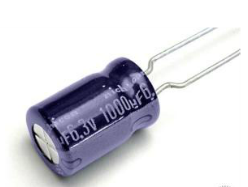
\includegraphics[width=0.5\linewidth]{img/exp2/1}
				\caption{Electrolytic Capacitor}
				\label{fig:6}
			\end{figure}
			
			Electrolytic capacitors (Figure \ref{fig:6}) are polarized and they must be connected the correct way round , atleast one of their leads will be marked $+$ or $–$. It is very easy to find the values of electrolytic capacitors because they are clearly printed with their capacitance and voltage rating.
			
		\subsubsection{Tantalum Capacitor}
			\begin{figure}[h]
				\centering
				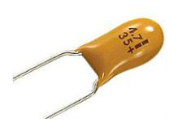
\includegraphics[width=0.5\linewidth]{img/exp2/6}
				\caption{Tantalum Capacitor}
				\label{fig:7}
			\end{figure}
		
			Tantalum bead capacitors (Figure \ref{fig:7}) are polarized and have low voltage ratings like electrolytic capacitors . Usually , the $+$ symbol is used to show the positive component lead . Modern tantalum bead capacitors are printed with their capacitance voltage and polarity in full. However older ones use a color–code system which has two stripes (for the two digits) and a spot of color for the number of zeros to give the value in $\mu F$.
			
		\subsubsection{Un-polarized Capacitors - small values (upto $1\mu F$)}
			\begin{figure}[h]
				\centering
				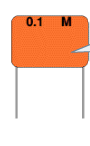
\includegraphics[width=0.2\linewidth]{img/exp2/7}
				\caption{Numbers printed on un-polarized capacitor}
				\label{fig:8}
			\end{figure}
			
			The value printed but without a multiplier, so you need to use experience to work out what the multiplier should be! For example $0.1$ means $0.1pF$. Sometimes the multiplier is used in place of the decimal point: For example: $4n7$ means $4.7nF$.
		
		\subsubsection{Un-polarized Capacitors - Capacitor Number Code}			
			\begin{figure}[ht]
				\centering 
				\subfloat[Codes printed on un-polarized capacitor]{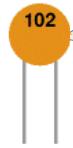
\includegraphics[width=0.2\textwidth,valign=c]{img/exp2/8}
					\label{fig:numCaps:1}}	
				\hfill
				\subfloat[Color coded un-polarized capacitors]{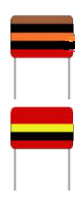
\includegraphics[width=0.2\textwidth,valign=c]{img/exp2/9}
					\label{fig:numCaps:2}}			
				\caption{\textit{Different ways of printing its capacitance on capacitors}}
			\end{figure}
		
			A number code (Figure \ref{fig:numCaps:1}) is often used on small capacitors where printing is difficult: The 1st number is the 1st digit, the 2nd number is the 2nd digit, the 3rd number is the number of zeros to give the capacitance in $pF$. Ignore any letters - they just indicate tolerance and voltage rating. For example: $102$ means $1000pF$ (not $102pF$) For example: $472J$ means $4700pF$ (J means 5\% tolerance).
			
			A color code was used on polyester capacitors for many years (Figure \ref{fig:numCaps:2}). It is now obsolete, but of course there are many still around. The colors should be read like the resistor code, the top three color bands giving the value in $pF$. Ignore the $4^{th}$ band (tolerance) and $5^{th}$ band (voltage rating). For example: brown, black, orange means $10000pF$. Note that there are no gaps between the color bands, so 2 identical bands actually appear as a wide band. For example: wide red, yellow means $220nF$.
			
		\subsection{Capacitors in series}
			\begin{figure}[h]
				\centering
				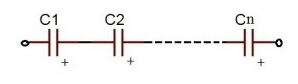
\includegraphics[width=0.5\linewidth]{img/exp2/10}
				\caption{Capacitor in series}
				\label{fig:capsInSeries}
			\end{figure}
		
			Capacitors in series means two or more capacitors connected in a single line. Positive plate of the one capacitor is connected to the negative plate of the next capacitor.
			\begin{align*}
				Q_T &= Q_1 = Q_2 = \ldots = Q \\
				I_C &= I_1 = I_2 = \ldots = I
			\end{align*}
			where,\\
			$Q_T$ is the total charge,\\
			$I_C$ is the capacitive current
			
			When the capacitors are connected in series Charge and current is same on all the capacitors.
			
			For series capacitors same quantity of electrons will flow through each capacitor because the charge on each plate is coming from the adjacent plate. So, coulomb charge is same. As current is nothing but flow of electrons, current is also same.
			
			
			Equivalent Capacitance for two capacitors in series,
			\begin{align*}
				\frac{1}{C_{eq}} &= \frac{1}{C_1} + \frac{1}{C_2} \\
				\frac{1}{C_{eq}} &= \frac{C_1 C_2}{C_1 + C_2}
			\end{align*}
		
		\subsection{Capacitors in parallel}
			\begin{figure}[h]
				\centering
				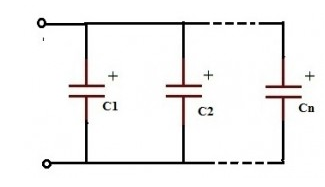
\includegraphics[width=0.5\linewidth]{img/exp2/11}
				\caption{Capacitor in parallel}
				\label{fig:capsInParallel}
			\end{figure}
			When the capacitors are connected in parallel the total capacitance value is increased. There are some applications where higher capacitance values are required.
			
			All the capacitors which are connected in parallel have the same voltage and is equal to the $V_T$ applied between the input and output terminals of the circuit.
			\begin{align*}
				V_T &= V_1 = V_2
			\end{align*}
			
			Equivalent Capacitance for two capacitors in parallel,
			\begin{align*}
				C_{eq} &= C_1 + C_2
			\end{align*}
		
	\section{Procedure}
		\subsection{Functioning of Capacitor}
			\begin{figure}[ht]
				\centering 
				\subfloat[Circuit with no capacitor]{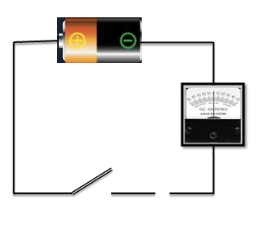
\includegraphics[width=0.3\textwidth,valign=c]{img/exp2/12}
					\label{fig:working:1}}
				\hfill
				\subfloat[Circuit with 2-step key and 1 ammeter]{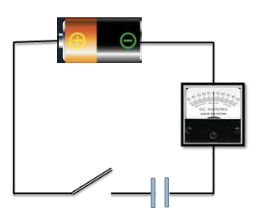
\includegraphics[width=0.3\textwidth,valign=c]{img/exp2/14}
					\label{fig:working:2}}		
				\hfill
				\subfloat[Circuit with 2-step key and 2 ammeter]{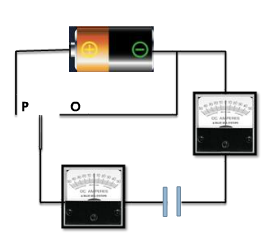
\includegraphics[width=0.3\textwidth,valign=c]{img/exp2/13}
					\label{fig:working:3}}			
				\caption{\textit{Understanding of working of capacitor using different circuits}}
			\end{figure}
			
			\begin{enumerate}
				\tightlist
				\item Consider a circuit set up like in the Figure \ref{fig:working:1}. The Ammeter will show a reading of $0$.
				\item Now let’s place large metal plate at each of the connectors a few millimetres apart as in Figure \ref{fig:working:2}. The Ammeter will flick on one side and come back to $0$.
				\item Let us extend this by placing a galvanometer on both sides of the capacitor and using a two-way switch as in Figure \ref{fig:working:3}. When the switch is connected to $P$, both the ammeters flick briefly to right.
				\item After moving to $P$ now the switch is moved to $O$. For both of the Ammeters, both flick briefly to left.
				\item Instead of moving to $P$ the first time, if the switch is first moved to $O$, neither Ammeters moves.
				\item The behaviour of the ammeter needles in the previous experiment suggests that a current flow firstly one way, then the other as the switch is moved from P to O. So, this suggests equal amounts of charge flows off one plate and onto the other
			\end{enumerate}							
			
		\subsection{Charging and Discharging}
			We say that the capacitor is charged up when connected to $P$ and discharged when moved to $O$.
			
			\begin{figure}[ht]
				\centering 
				\subfloat[capacitor connected to a battery]{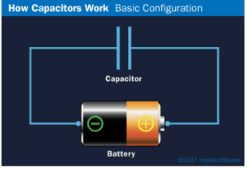
\includegraphics[width=0.3\textwidth,valign=c]{img/exp2/15}
					\label{fig:cd:1}}
				\hfill
				\subfloat[charging of a capacitor]{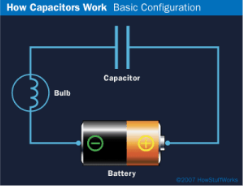
\includegraphics[width=0.3\textwidth,valign=c]{img/exp2/16}
					\label{fig:cd:2}}		
				\hfill
				\subfloat[discharging of a capacitor]{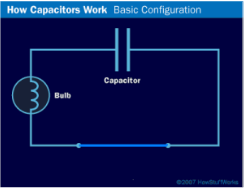
\includegraphics[width=0.3\textwidth,valign=c]{img/exp2/17}
					\label{fig:cd:3}}			
				\caption{\textit{Understanding of charging and discharging of a capacitor using different circuits}}
			\end{figure}				
			
			\subsubsection{Charging}					
				The plate on the capacitor that attaches to the negative terminal of the battery accepts electrons that the battery is producing .The plate on the capacitor that attaches to the positive terminal of the battery loses electrons to the battery. Once it’s charged , the capacitor has the sam voltage as the battery. (This is in reference to Figure \ref{fig:cd:1})
				
				Now, we connect a bulb to the circuit as per Figure \ref{fig:cd:2}. The bulb will first glow and then keep dimming and finally turn off.
				
			\subsubsection{Discharging}
				If you then remove the battery and replace it with a wire , current will flow from one plate of the capacitor to the other. The bulb will light initially and then dim as the capacitor discharges , until it is completely out. (This is in reference to Figure \ref{fig:cd:3})

	\section{Conclusion}
		Capacitors are common elements of electrical networks and electronic circuits and are ubiquitous in electronic equipment. The electrical function of a capacitor is specified by its capacitance: common commercial capacitors are manufactured over a wide variety of types. The nominal value of the capacitance falls within the manufacturing tolerance, indicated on the component.